% =================================================================================================
% File:			server_tier/endpoints.tex
% Description:	Definisce la sezione relativa al back-end dell'applicazione
% Created:		2015-04-07
% Author:		Cusinato Giacomo
% Email:		cusinato.giacomo@mashup-unipd.it
% =================================================================================================
% Modification History:
% Version		Modifier Date		Change											Author
% 0.0.1
% =================================================================================================

% CONTENUTO DEL CAPITOLO


\subsubsection{server::endpoints} % (fold)
\label{ssub:bdsm_app_server_endpoints}
\begin{figure}[!htbp]
	\centering
	\centerline{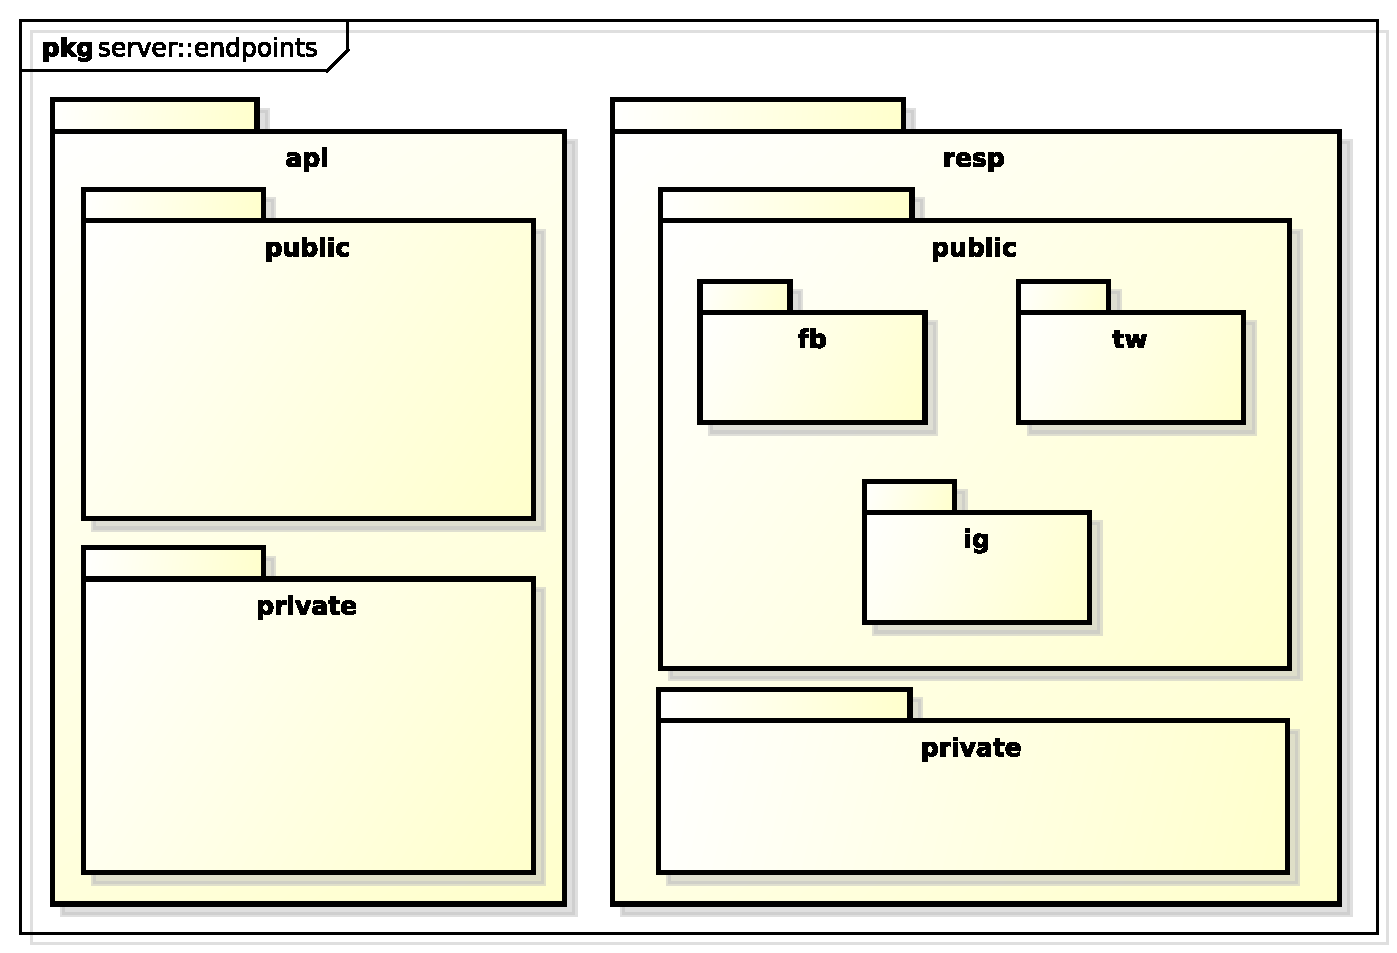
\includegraphics[scale=0.6]{./images/server/endpoints.pdf}}
	\caption{Package - server::endpoints}
\end{figure}

\begin{itemize}
  \item \textbf{Descrizione}: è il package che contiene tutte le classi che implementato l'interfaccia REST del sistema tramite Google Cloud Endpoints;
  \item \textbf{Padre}: server
  \item \textbf{Package contenuti}:
  	\begin{itemize}
  		\item server::endpoints::api
  		\item server::endpoints::resp
	\end{itemize}
  \item \textbf{Interazione con altri componenti}:
  	\begin{itemize}
  		\item server::processor
  		\item server::db
	\end{itemize}
\end{itemize}
% subsubsection

\subsubsection{server::endpoints::api} % (fold)
\label{ssub:bdsm_app_server_endpoints_api}

	In questo package e nei suoi package figli viene utilizzata la classe \textbf{ResourceContainer} offerta dai Google Cloud Endpoints per le richieste contenenti percorsi e query.
\begin{figure}[!htbp]
	\centering
	\centerline{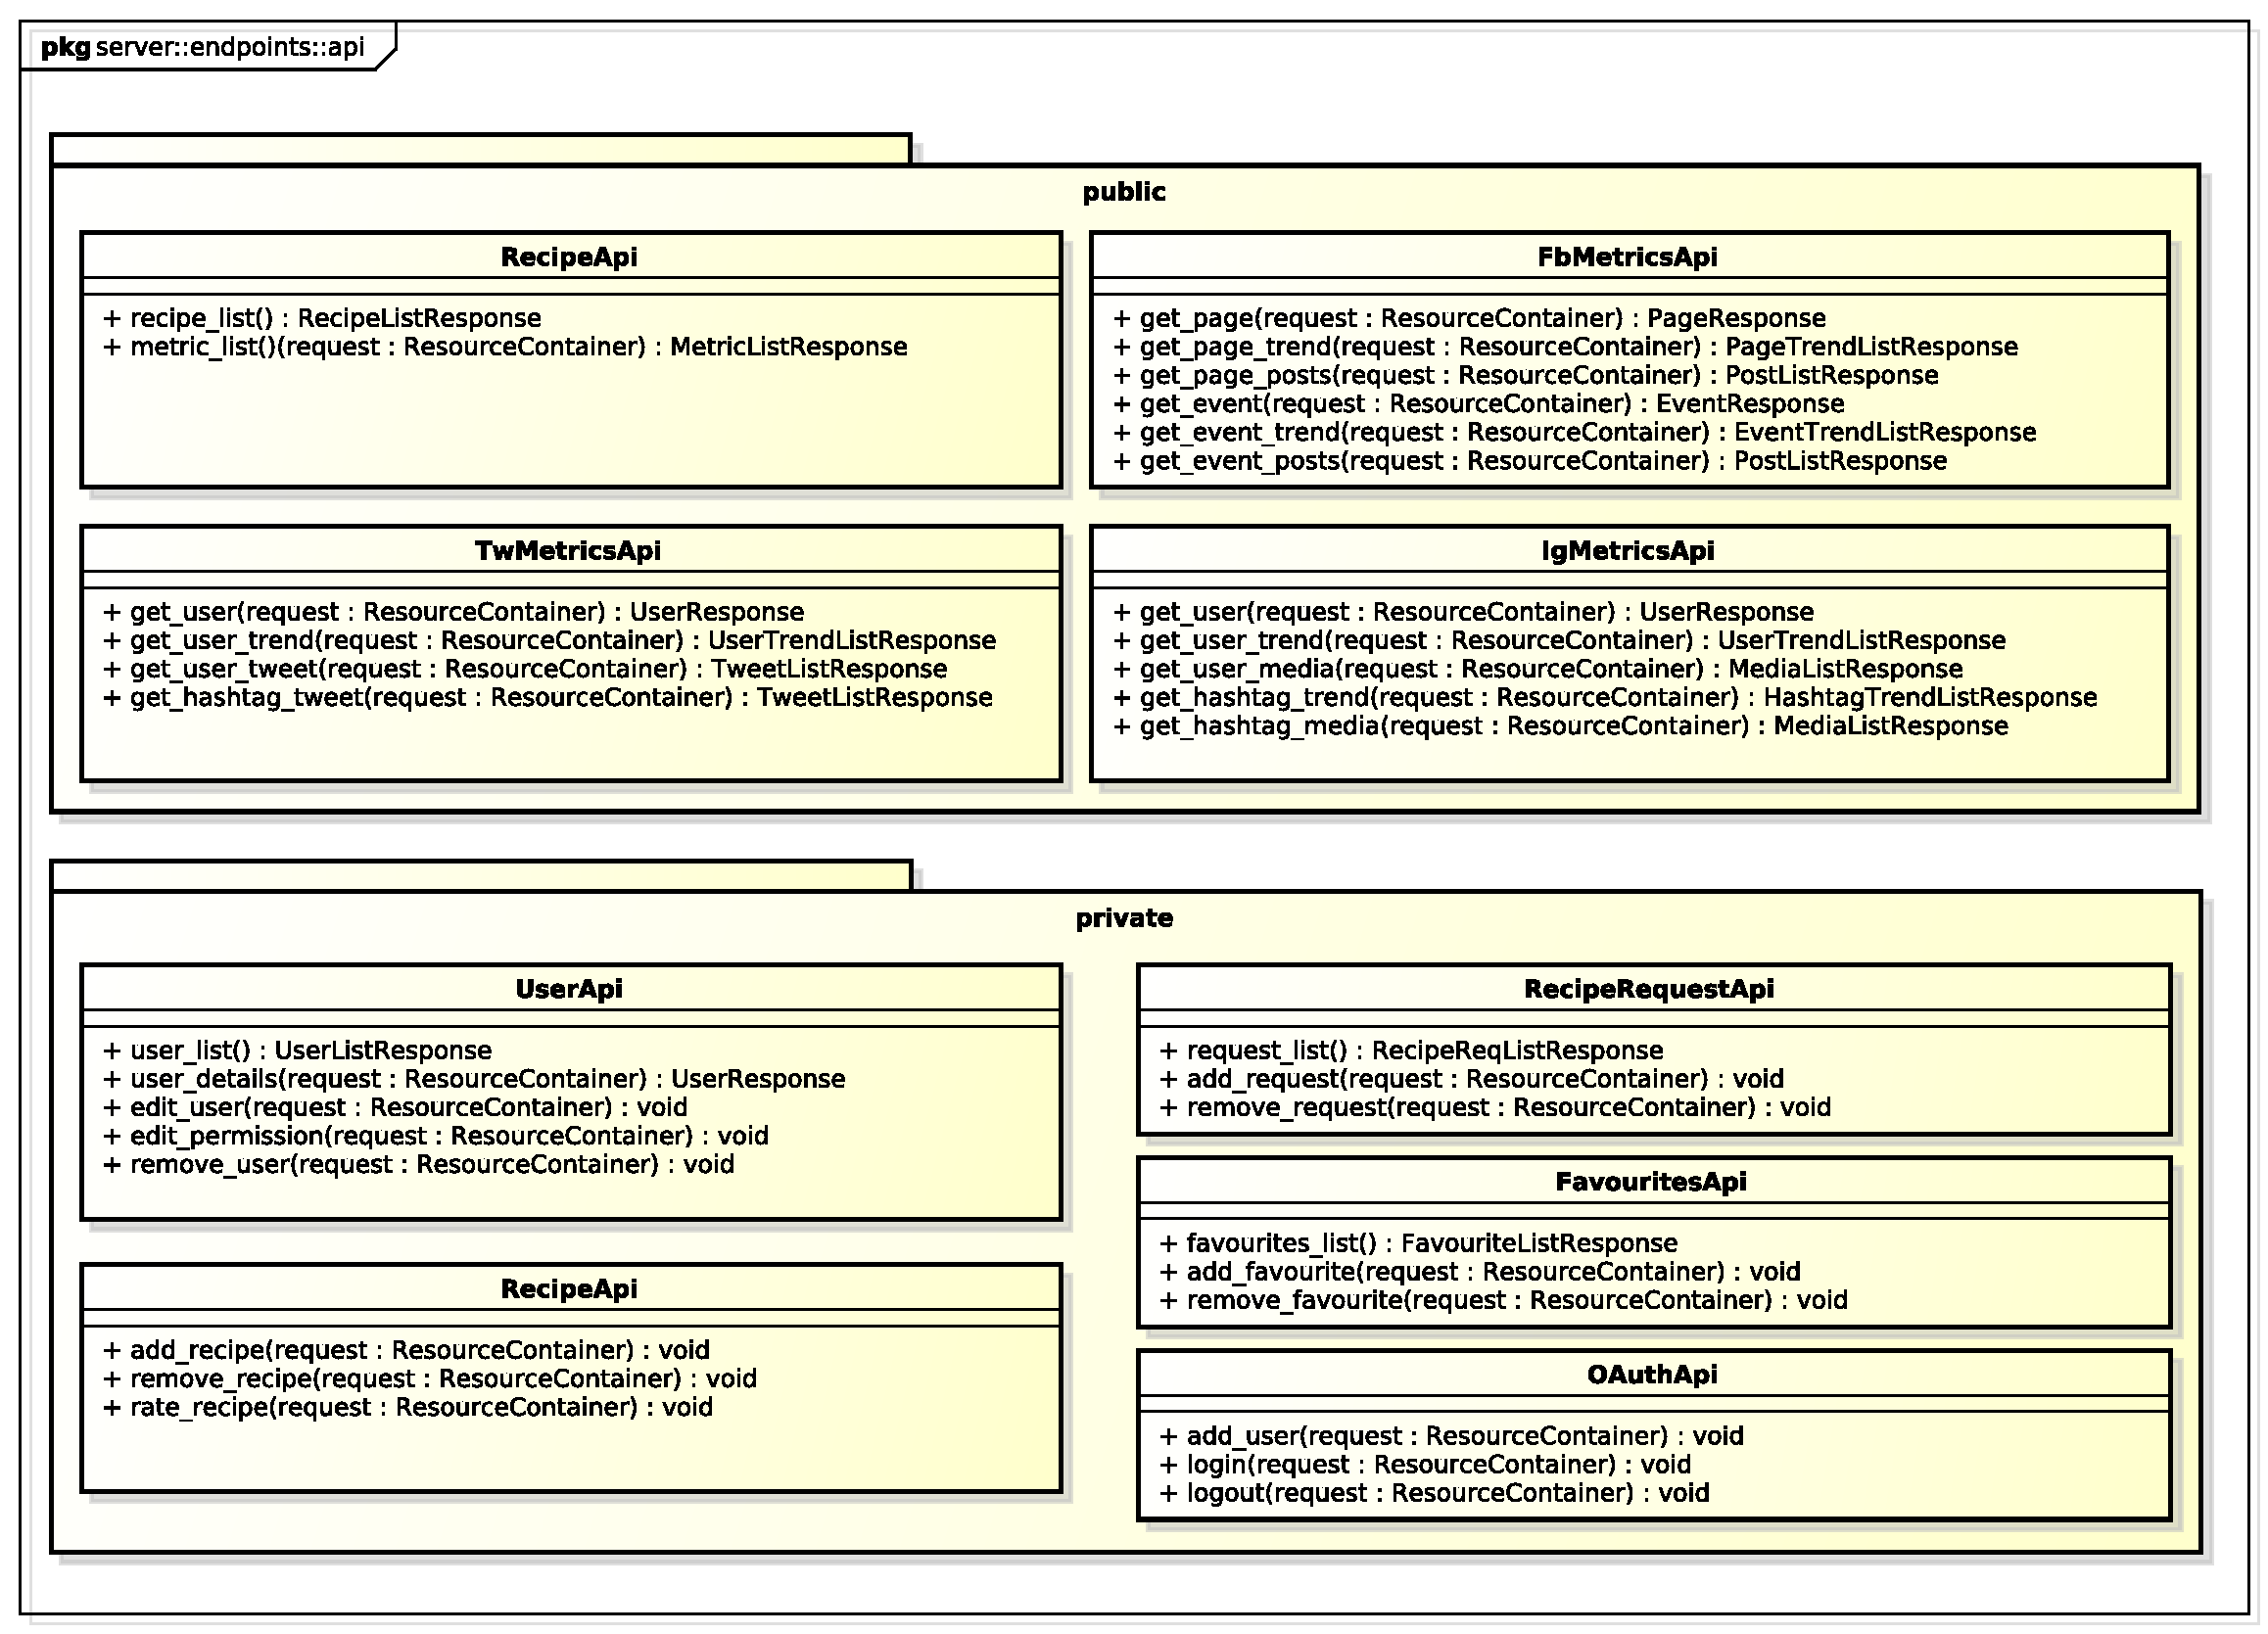
\includegraphics[scale=0.4]{./images/server/api.pdf}}
	\caption{Package - server::endpoints::api}
\end{figure}

\begin{itemize}
  \item \textbf{Descrizione}: è il package che definisce le web API offerte dall'applicazione e utilizzati dal client;
  \item \textbf{Padre}: server::endpoints
  \item \textbf{Package contenuti}:
  	\begin{itemize}
  		\item server::endpoints::api::public
  		\item server::endpoints::api::private
	\end{itemize}
  \item \textbf{Interazione con altri componenti}:
  	\begin{itemize}
  		\item client::model::services
  		\item server::processor
  		\item server::db
			\item server::endpoints::resp
	\end{itemize}
\end{itemize}
% subsubsection

\subsubsection{server::endpoints::api::public} % (fold)
\label{ssub:bdsm_app_server_endpoints_api_public}
\begin{figure}[!htbp]
	\centering
	\centerline{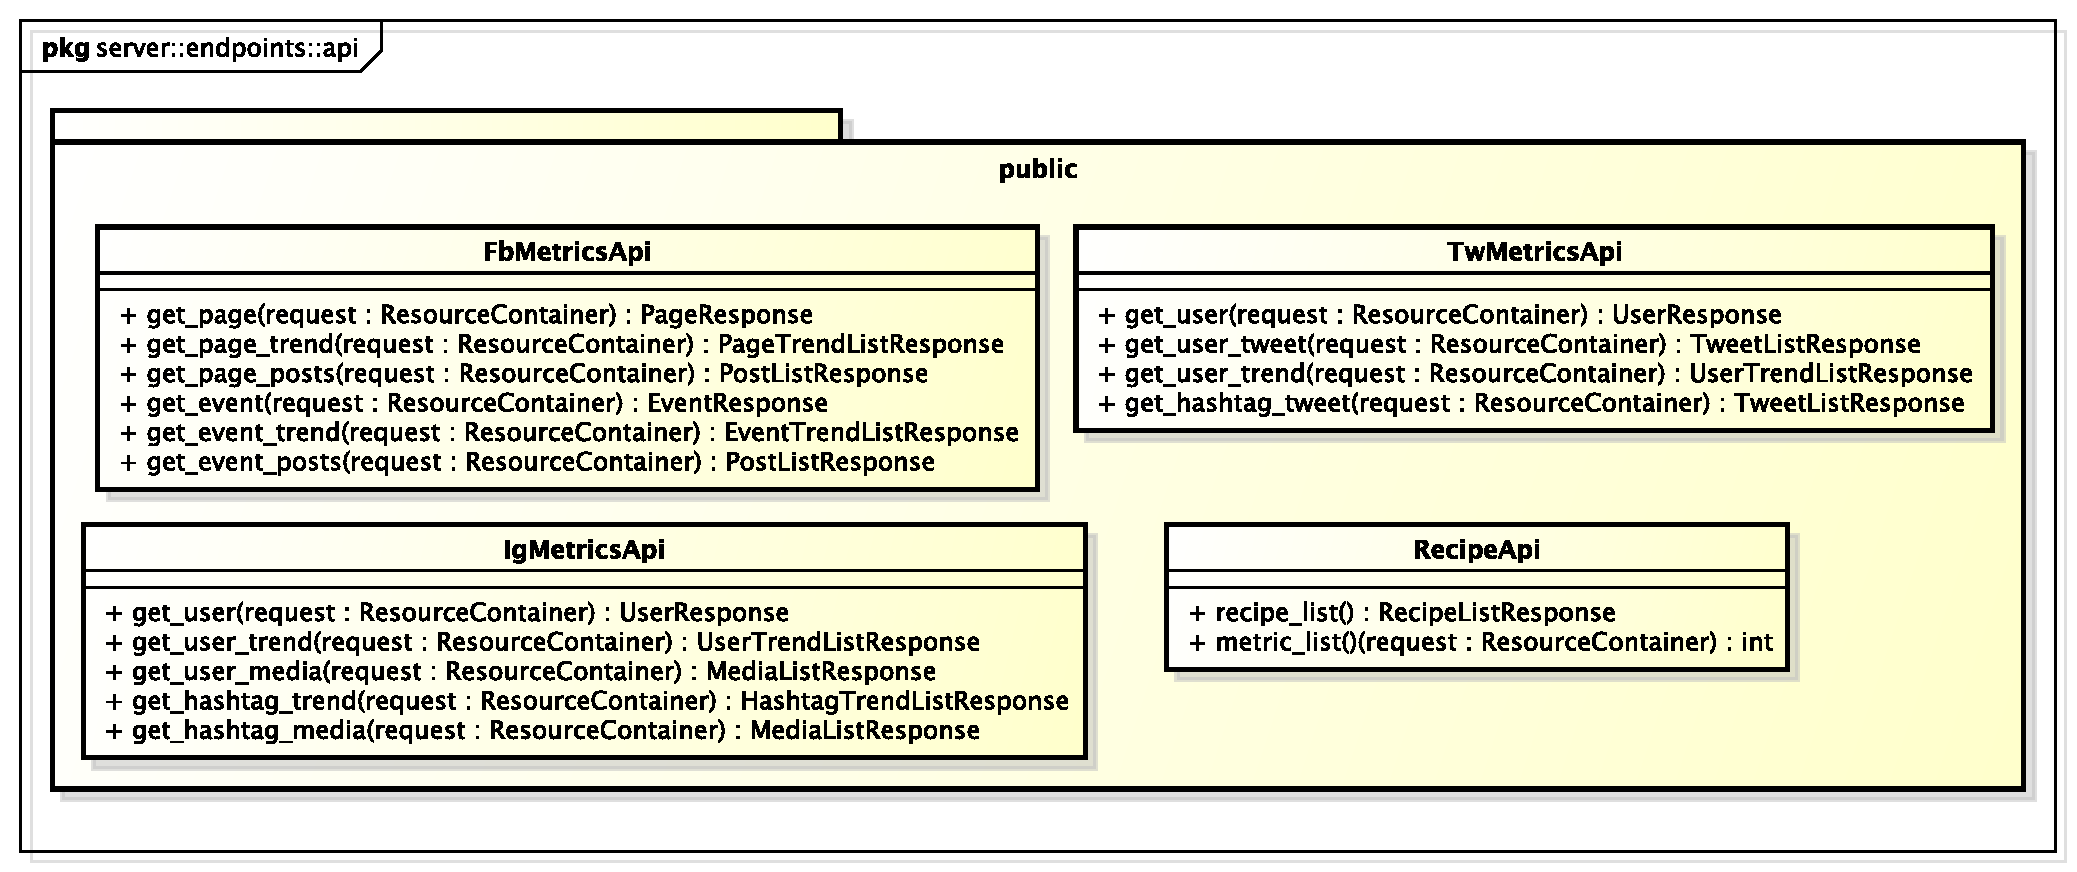
\includegraphics[scale=0.4]{./images/server/api_public.pdf}}
	\caption{Package - server::endpoints::api::public}
\end{figure}

\begin{itemize}
  \item \textbf{Descrizione}: è il package contenente l'implementazione delle web API pubbliche;
  \item \textbf{Padre}: server::endpoints::api
  \item \textbf{Interazione con altri componenti}:
  	\begin{itemize}
        \item server::processor
				\item server::endpoints::resp::public
    \end{itemize}
\end{itemize}
% subsubsection

	\paragraph{Classi} % (fold)

    \subparagraph{server::endpoints::api::public::RecipeApi} % (fold)
    \label{subp:bdsm_app_server_endpoints_api_public_recipeapi}
    \begin{itemize}
      \item \textbf{Descrizione}: classe utilizzata in seguito ad una chiamata del client per ricavare la lista delle Recipe e delle metriche;
      \item \textbf{Utilizzo}: i suoi metodi vengono invocati quando viene richiesto dal client di recuperare la lista delle Recipe e delle metriche;
      \item \textbf{Relazioni con altre classi}:
        \begin{itemize}
          \item server::endpoints::resp::public::MetricListResponse;
          \item server::endpoints::resp::private::RecipeListResponse;
        \end{itemize}
      \end{itemize}
    % subparagraph bdsm_app_server_endpoints_api_public_recipeapi (end)

    \subparagraph{server::endpoints::api::public::FbMetricsApi} % (fold)
    \label{subp:bdsm_app_server_endpoints_api_public_fbmetricsapi}
    \begin{itemize}
      \item \textbf{Descrizione}: classe utilizzata in seguito ad una chiamata del client per ottenere i dati relativi ad una metrica di Facebook;
      \item \textbf{Utilizzo}: i suoi metodi vengono invocati quando viene richiesto dal client dei dati relativi ad una pagina o ad un evento di Facebook;
      \item \textbf{Relazioni con altre classi}:
        \begin{itemize}
          \item server::endpoints::resp::public::fb::PageResponse
          \item server::endpoints::resp::public::fb::PageTrendListResponse
          \item server::endpoints::resp::public::fb::PostListResponse
          \item server::endpoints::resp::public::fb::EventResponse
          \item server::endpoints::resp::public::fb::EventTrendListResponse
        \end{itemize}
      \end{itemize}
    % subparagraph bdsm_app_server_endpoints_api_public_fbmetricsapi (end)

    \subparagraph{server::endpoints::api::public::TwMetricsApi} % (fold)
    \label{subp:bdsm_app_server_endpoints_api_public_twmetricsapi}
    \begin{itemize}
      \item \textbf{Descrizione}: classe utilizzata in seguito ad una chiamata del client per ottenere i dati relativi ad una metrica di Twitter;
      \item \textbf{Utilizzo}: i suoi metodi vengono invocati quando viene richiesto dal client dei dati relativi ad un utente o un hashtag di Twitter;
      \item \textbf{Relazioni con altre classi}:
        \begin{itemize}
          \item server::endpoints::resp::public::tw::UserResponse
          \item server::endpoints::resp::public::tw::UserTrendListResponse
          \item server::endpoints::resp::public::tw::TweetListResponse
        \end{itemize}
      \end{itemize}
    % subparagraph bdsm_app_server_endpoints_api_public_twmetricsapi (end)

    \subparagraph{server::endpoints::api::public::IgMetricsApi} % (fold)
    \label{subp:bdsm_app_server_endpoints_api_public_igmetricsapi}
    \begin{itemize}
      \item \textbf{Descrizione}: classe utilizzata in seguito ad una chiamata del client per ottenere i dati relativi ad una metrica di Instagram;
      \item \textbf{Utilizzo}: i suoi metodi vengono invocati quando viene richiesto dal client dei dati relativi ad un utente o hashtag di Instagram;
      \item \textbf{Relazioni con altre classi}:
        \begin{itemize}
          \item server::endpoints::resp::public::ig::UserResponse
          \item server::endpoints::resp::public::ig::UserTrendListResponse
          \item server::endpoints::resp::public::ig::MediaListResponse
          \item server::endpoints::resp::public::ig::HashtagTrendListResponse
        \end{itemize}
      \end{itemize}
    % subparagraph bdsm_app_server_endpoints_api_public_igmetricsapi (end)

\subsubsection{server::endpoints::api::private} % (fold)
\label{ssub:bdsm_app_server_endpoints_api_private}
\begin{figure}[!htbp]
	\centering
	\centerline{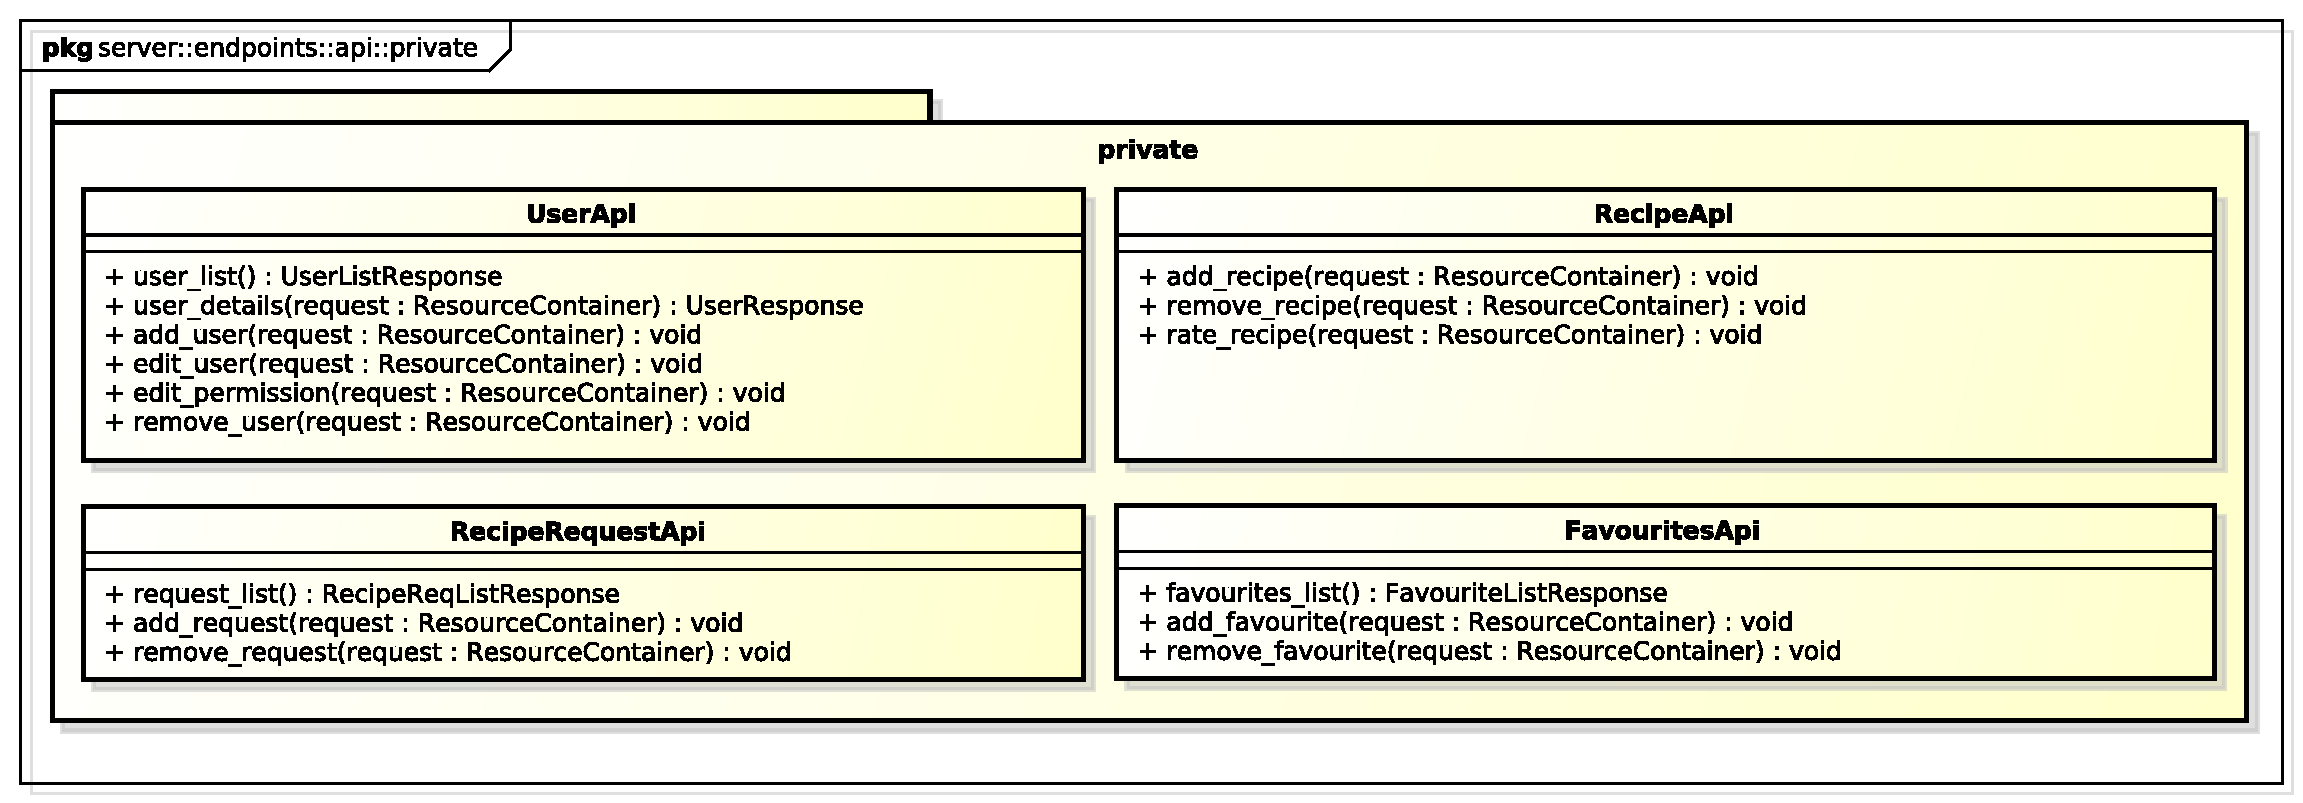
\includegraphics[scale=0.4]{./images/server/api_private.pdf}}
	\caption{Package - server::endpoints::api::private}
\end{figure}

\begin{itemize}
  \item \textbf{Descrizione}: è il package contenente l'implementazione delle web API private;
  \item \textbf{Padre}: server::endpoints::api
  \item \textbf{Interazione con altri componenti}:
  	\begin{itemize}
        \item server::processor
				\item server::endpoints::resp::private
    \end{itemize}
\end{itemize}
% subsubsection

	\paragraph{Classi} % (fold)

    \subparagraph{server::endpoints::api::private::RecipeApi} % (fold)
    \label{subp:bdsm_app_server_endpoints_api_private_recipeapi}
    \begin{itemize}
      \item \textbf{Descrizione}: classe che rappresenta l'implementazione delle web API relative alla gestione delle Recipe;
      \item \textbf{Utilizzo}: i suoi metodi vengono invocati quando viene richiesto dal client di aggiungere, rimuovere o valutare una Recipe;
      \item \textbf{Relazioni con altre classi}:
        \begin{itemize}
          \item server::endpoints::resp::private::RecipeListResponse
        \end{itemize}
      \end{itemize}
    % subparagraph bdsm_app_server_endpoints_api_private_recipeapi (end)

    \subparagraph{server::endpoints::api::private::UserApi} % (fold)
    \label{subp:bdsm_app_server_endpoints_api_private_userapi}
    \begin{itemize}
      \item \textbf{Descrizione}: classe che rappresenta l'implementazione delle web API relative alla gestione degli utenti;
      \item \textbf{Utilizzo}: i suoi metodi vengono invocati quando viene richiesto dal client di aggiungere o rimuovere un utente, ricavare o modificare i dati di un utente o per modificare i dati di un utente;
      \item \textbf{Relazioni con altre classi}:
        \begin{itemize}
          \item server::endpoints::resp::private::UserResponse
        \end{itemize}
      \end{itemize}
    % subparagraph bdsm_app_server_endpoints_api_private_userapi (end)

    \subparagraph{server::endpoints::api::private::RecipeRequestApi} % (fold)
    \label{subp:bdsm_app_server_endpoints_api_private::reciperequestapi}
    \begin{itemize}
      \item \textbf{Descrizione}: classe che rappresenta l'implementazione delle web API relative alla gestione delle richieste di aggiunta Recipe;
      \item \textbf{Utilizzo}: i suoi metodi vengono invocati quando viene inviata una richiesta di nuova Recipe o la rimozione di una richiesta esistente da parte del client;
      \item \textbf{Relazioni con altre classi}:
        \begin{itemize}
          \item server::endpoints::resp::private::RecipeReqListResponse
        \end{itemize}
      \end{itemize}
    % subparagraph bdsm_app_server_endpoints_api_private_reciperequestapi (end)

    \subparagraph{server::endpoints::api::private::FavoritesApi} % (fold)
    \label{subp:bdsm_app_server_endpoints_api_private_favoritesapi}
    \begin{itemize}
      \item \textbf{Descrizione}: classe che rappresenta l'implementazione delle web API relative alla gestione delle View preferite per ogni utente;
      \item \textbf{Utilizzo}: i suoi metodi vengono invocati quando viene richiesto dal client l'inserimento di una View nei preferiti o quando viene richiesta la rimozione di una View aggiunta in precedenza;
      \item \textbf{Relazioni con altre classi}:
        \begin{itemize}
          \item server::endpoints::resp::private::FavoriteListResponse
        \end{itemize}
      \end{itemize}
    % subparagraph bdsm_app_server_endpoints_api_private_favoritesapi (end)

\subsubsection{server::endpoints::resp} % (fold)
\label{ssub:bdsm_app_server_endpoints_resp}
\begin{figure}[!htbp]
	\centering
	\centerline{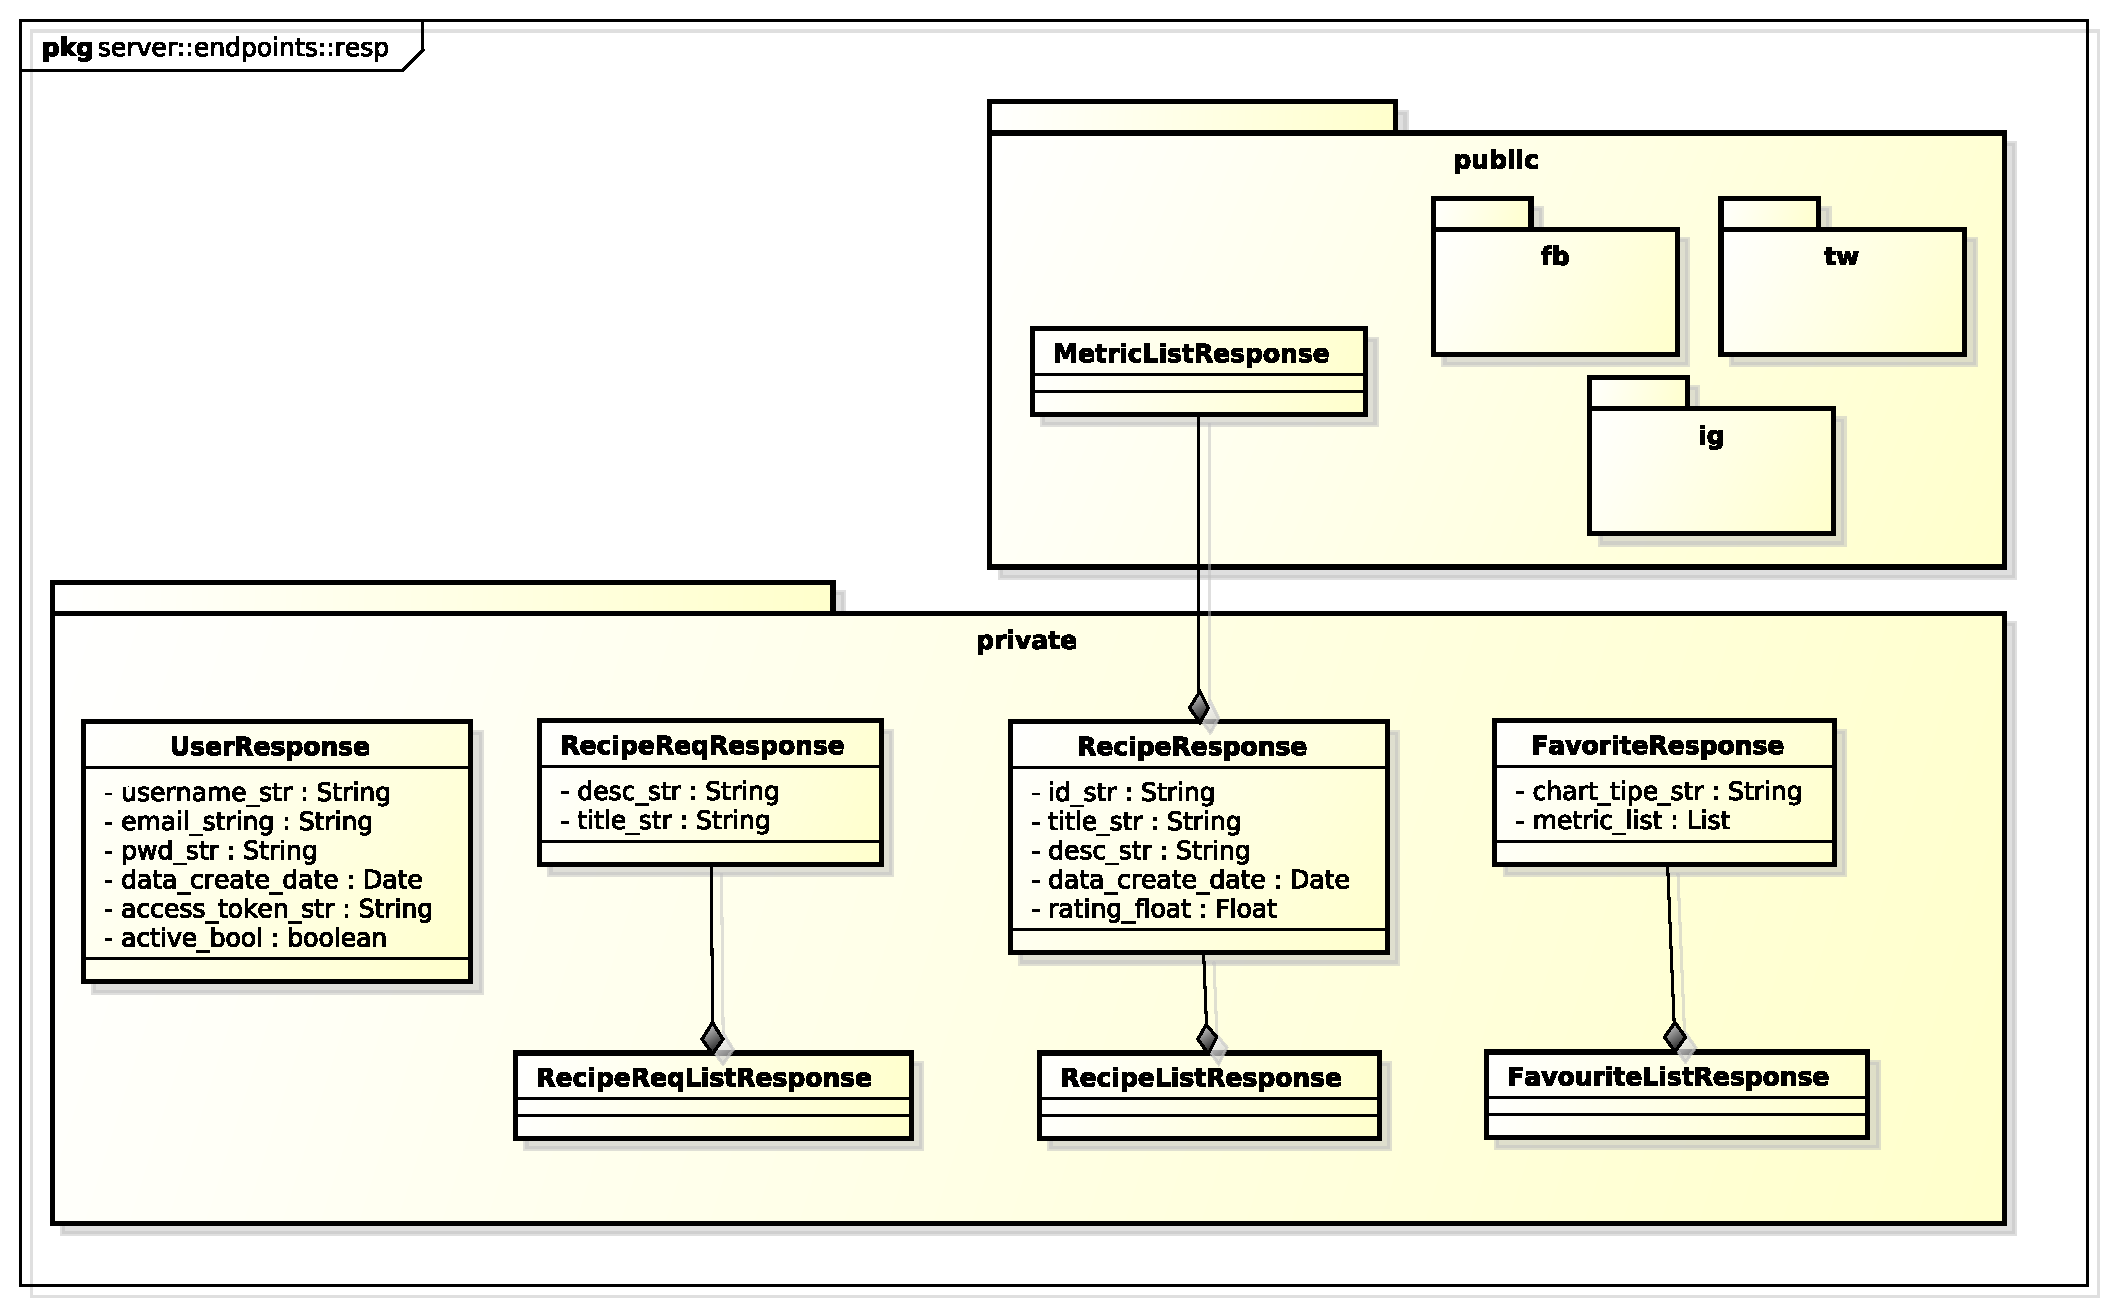
\includegraphics[scale=0.45]{./images/server/resp.pdf}}
	\caption{Package - server::endpoints::resp}
\end{figure}

\begin{itemize}
  \item \textbf{Descrizione}: è il package che definisce il modelli delle risposte da passare al client in seguito alle chiamate API;
  \item \textbf{Padre}: server::endpoints
  \item \textbf{Package contenuti}:
  	\begin{itemize}
  		\item server::endpoints::resp::public
  		\item server::endpoints::resp::private
	\end{itemize}
\end{itemize}
% subsubsection

\subsubsection{server::endpoints::resp::public} % (fold)
\label{ssub:bdsm_app_server_endpoints_resp_public}
\begin{figure}[!htbp]
	\centering
	\centerline{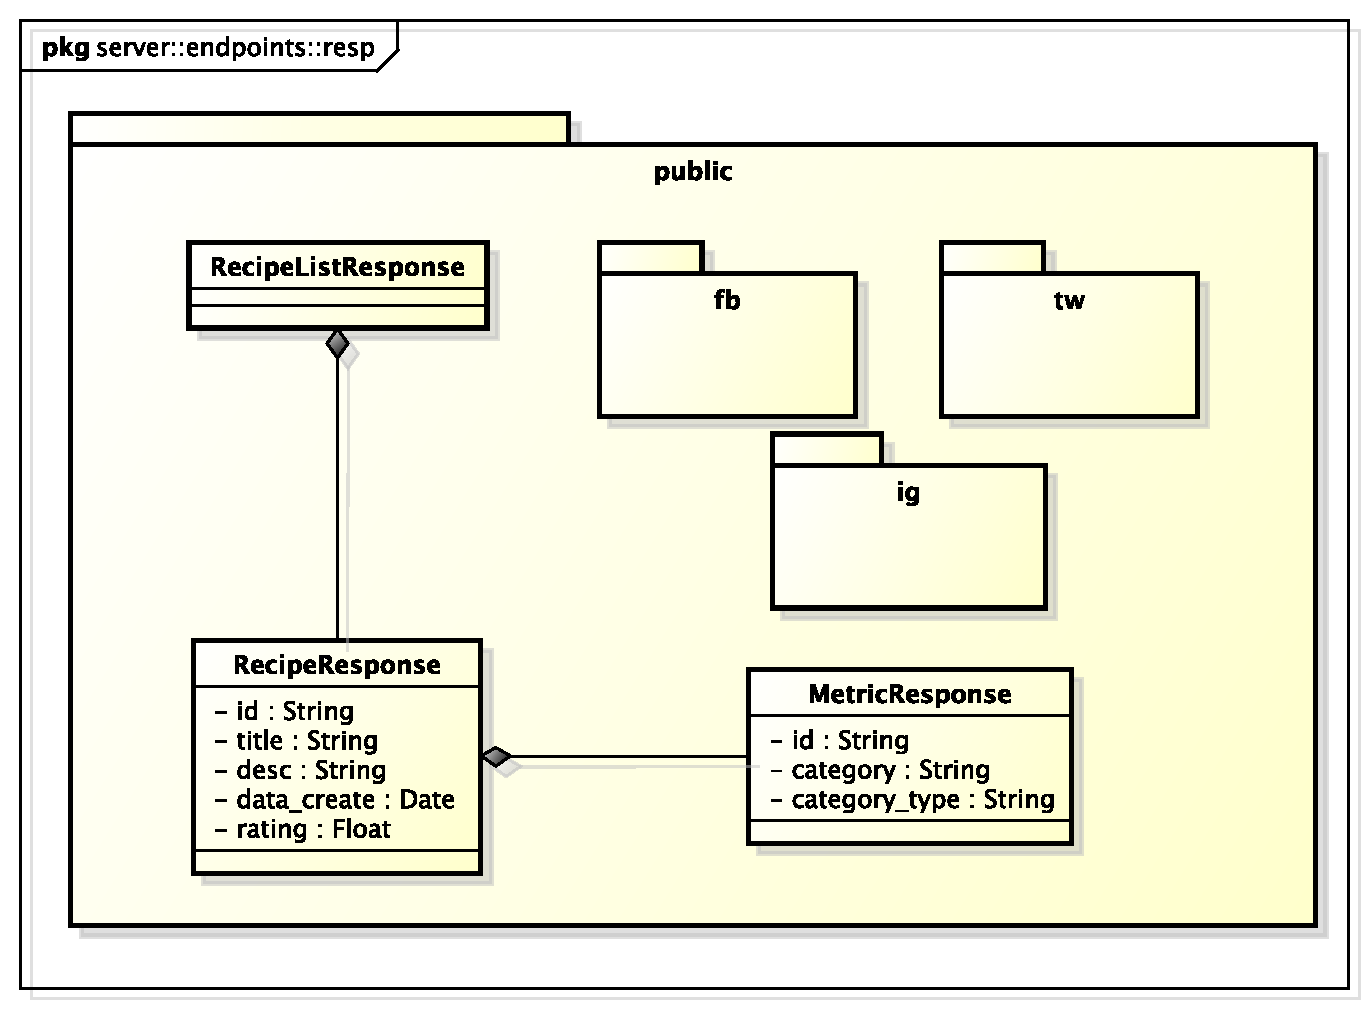
\includegraphics[scale=0.55]{./images/server/resp_public.pdf}}
	\caption{Package - server::endpoints::resp::public}
\end{figure}

\begin{itemize}
  \item \textbf{Descrizione}: è il package che definisce il modello delle risposte da passare al client in seguito alle chiamate delle API pubbliche;
  \item \textbf{Padre}: server::endpoints::resp
  \item \textbf{Package contenuti}:
  	\begin{itemize}
  		\item server::endpoints::resp::public::fb
  		\item server::endpoints::resp::public::tw
  		\item server::endpoints::resp::public::ig
	\end{itemize}
  \item \textbf{Interazione con altri componenti}:
  	\begin{itemize}
  		\item server::endpoints::resp::private
	\end{itemize}
\end{itemize}
% subsubsection

	\paragraph{Classi} % (fold)

    \subparagraph{server::endpoints::resp::public::MetricListResponse} % (fold)
    \label{subp:bdsm_app_server_endpoints_resp_public_metriclistresponse}
    \begin{itemize}
      \item \textbf{Descrizione}: rappresenta il modello dei dati della lista di metriche da ritornare al client;
      \item \textbf{Utilizzo}: viene utilizzata dalle API per restituire la response della lista delle metriche relative ad un Recipe al client;
      \item \textbf{Relazioni con altre classi}:
        \begin{itemize}
          \item server::endpoints::resp::public::fb::PageResponse
          \item server::endpoints::resp::public::fb::EventResponse
          \item server::endpoints::resp::public::tw::UserResponse
          \item server::endpoints::resp::public::tw::HashtagResponse
          \item server::endpoints::resp::public::ig::UserResponse
          \item server::endpoints::resp::public::ig::HashtagResponse
        \end{itemize}
      \end{itemize}
    % subparagraph bdsm_app_server_endpoints_resp_public_metriclistresponse (end)

\subsubsection{server::endpoints::resp::public::fb} % (fold)
\label{ssub:bdsm_app_server_endpoints_resp_public_fb}
\begin{figure}[!htbp]
	\centering
	\centerline{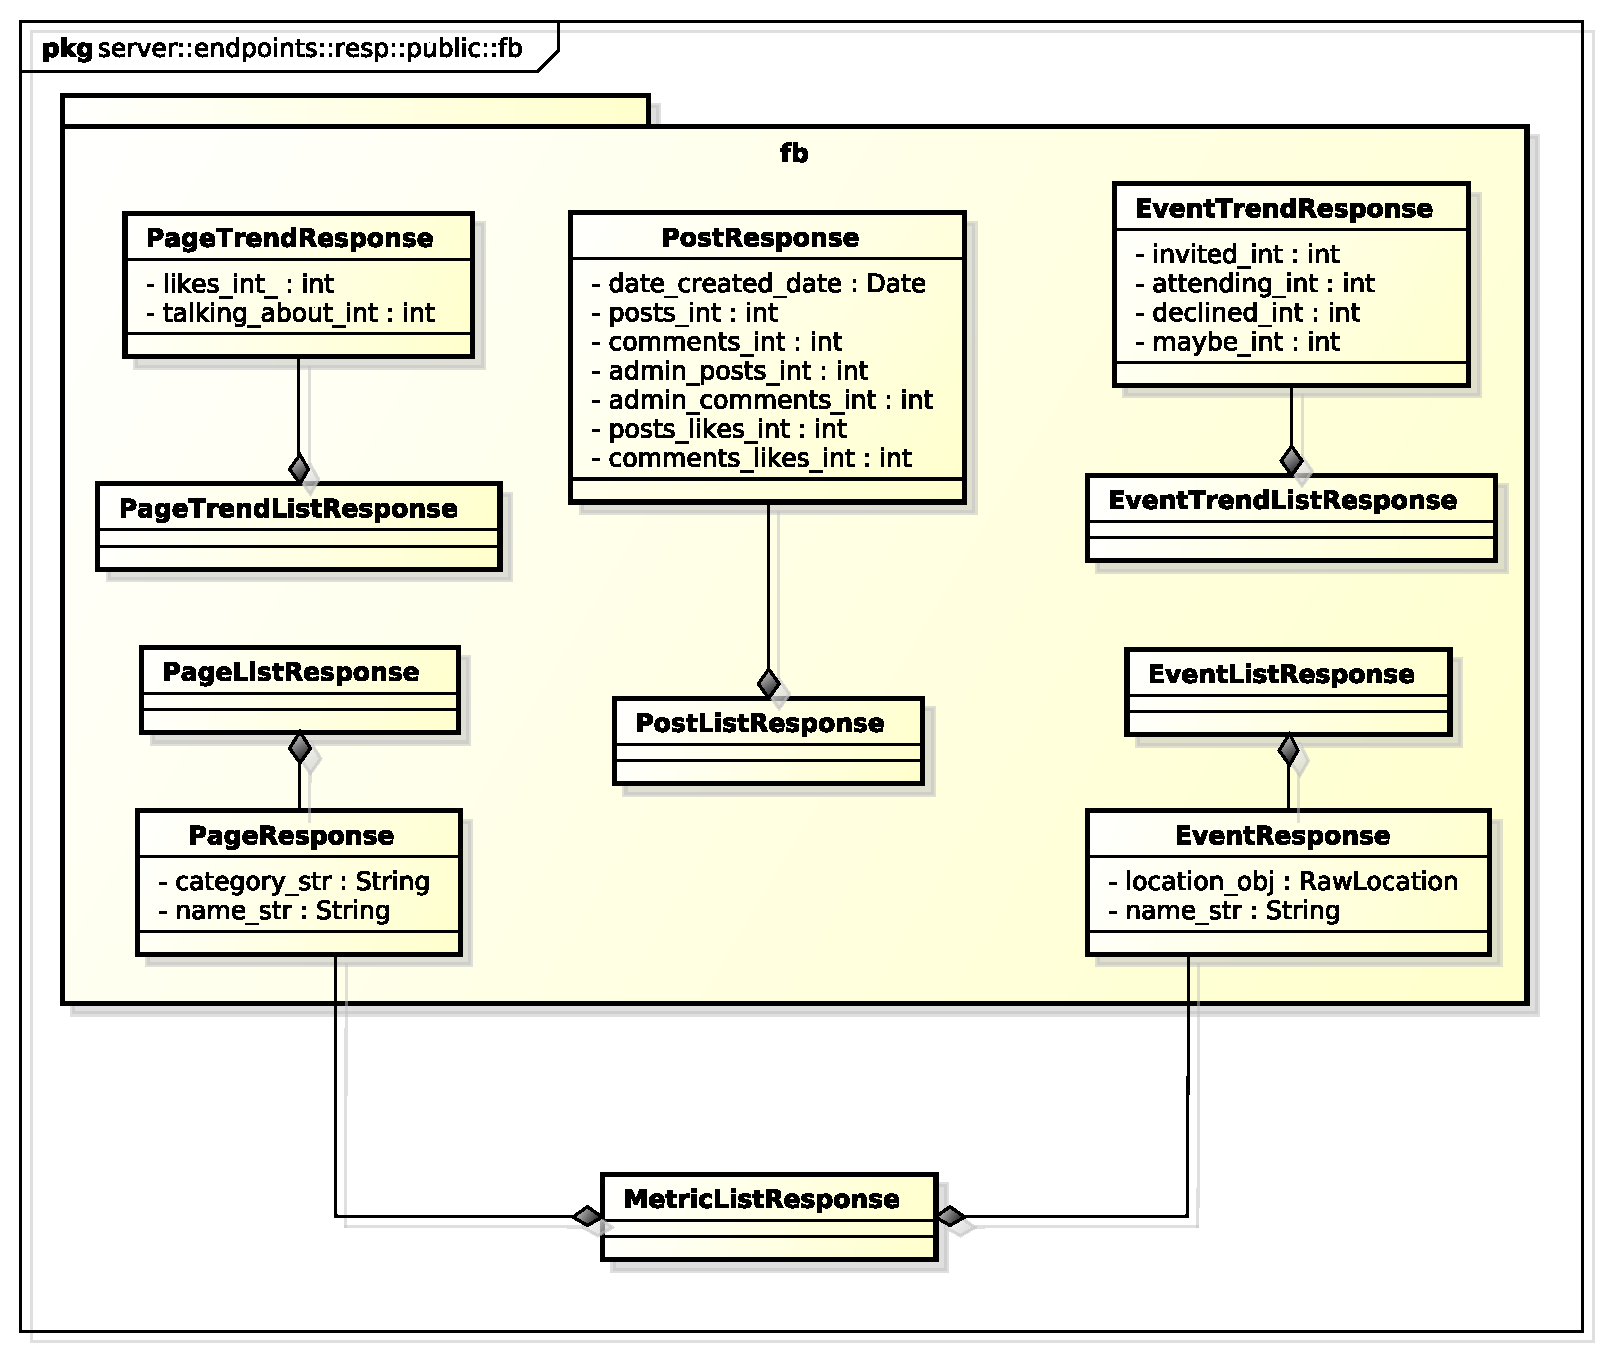
\includegraphics[scale=0.55]{./images/server/resp_fb.pdf}}
	\caption{Package - server::endpoints::resp::public::fb}
\end{figure}

\begin{itemize}
  \item \textbf{Descrizione}: è il package contenente le classi che rappresentano il modello di dati delle componenti di Facebook da restituire al client;
  \item \textbf{Padre}: server::endpoints::resp::public
  %\item \textbf{Interazione con altri componenti}:
\end{itemize}
% subsubsection

	\paragraph{Classi} % (fold)

    \subparagraph{server::endpoints::resp::public::fb::PageResponse} % (fold)
    \label{subp:bdsm_app_server_endpoints_resp_public_fb_pageresponse}
    \begin{itemize}
      \item \textbf{Descrizione}: rappresenta il modello dei dati di una pagina Facebook da ritornare al client;
      \item \textbf{Utilizzo}: viene utilizzata dalle API per restituire la response dei dati di una pagina Facebook al client;
      %\item \textbf{Relazioni con altre classi}:
      \end{itemize}
    % subparagraph bdsm_app_server_endpoints_resp_public_fb_pageresponse (end)

    \subparagraph{server::endpoints::resp::public::fb::PageListResponse} % (fold)
    \label{subp:bdsm_app_server_endpoints_resp_public_fb_pagelistresponse}
    \begin{itemize}
      \item \textbf{Descrizione}: rappresenta il modello dei dati della lista di pagine Facebook da ritornare al client;
      \item \textbf{Utilizzo}: viene utilizzata dalle API per restituire la response della lista delle pagine Facebook al client;
      \item \textbf{Relazioni con altre classi}:
        \begin{itemize}
          \item server::endpoints::resp::public::fb::PageResponse
        \end{itemize}
      \end{itemize}
    % subparagraph bdsm_app_server_endpoints_resp_public_fb_pagelistresponse (end)

    \subparagraph{server::endpoints::resp::public::fb::PageTrendResponse} % (fold)
    \label{subp:bdsm_app_server_endpoints_resp_public_fb_pagetrendresponse}
    \begin{itemize}
      \item \textbf{Descrizione}: rappresenta il modello dei dati dei trend di una pagina Facebook da ritornare al client;
      \item \textbf{Utilizzo}: viene utilizzata dalle API per restituire la response dei trend di una pagina Facebook al client;
      %\item \textbf{Relazioni con altre classi}:
      \end{itemize}
    % subparagraph bdsm_app_server_endpoints_resp_public_fb_pagetrendresponse (end)

    \subparagraph{server::endpoints::resp::public::fb::PageTrendListResponse} % (fold)
    \label{subp:bdsm_app_server_endpoints_resp_public_fb_pagetrendlistresponse}
    \begin{itemize}
      \item \textbf{Descrizione}: rappresenta il modello dei dati della lista dei trend di una pagina Facebook da ritornare al client;
      \item \textbf{Utilizzo}: viene utilizzata dalle API per restituire la response della lista dei trend di una pagina Facebook al client;
      \item \textbf{Relazioni con altre classi}:
        \begin{itemize}
          \item server::endpoints::resp::public::fb::PageTrendResponse
        \end{itemize}
      \end{itemize}
    % subparagraph bdsm_app_server_endpoints_resp_public_fb_pagetrendlistresponse (end)

    \subparagraph{server::endpoints::resp::public::fb::EventResponse} % (fold)
    \label{subp:bdsm_app_server_endpoints_resp_public_fb_eventresponse}
    \begin{itemize}
      \item \textbf{Descrizione}: rappresenta il modello dei dati di un evento di Facebook da ritornare al client;
      \item \textbf{Utilizzo}: viene utilizzata dalle API per restituire la response dei dati di un evento Facebook al client;
      %\item \textbf{Relazioni con altre classi}:
      \end{itemize}
    % subparagraph bdsm_app_server_endpoints_resp_public_fb_eventresponse (end)

    \subparagraph{server::endpoints::resp::public::fb::EventListResponse} % (fold)
    \label{subp:bdsm_app_server_endpoints_resp_public_fb_eventlistresponse}
    \begin{itemize}
      \item \textbf{Descrizione}: rappresenta il modello dei dati della lista di eventi Facebook da ritornare al client;
      \item \textbf{Utilizzo}: viene utilizzata dalle API per restituire la response della lista di eventi Facebook al client;
      \item \textbf{Relazioni con altre classi}:
        \begin{itemize}
          \item server::endpoints::resp::public::fb::EventResponse
        \end{itemize}
      \end{itemize}
    % subparagraph bdsm_app_server_endpoints_resp_public_fb_eventlistresponse (end)

    \subparagraph{server::endpoints::resp::public::fb::EventTrendResponse} % (fold)
    \label{subp:bdsm_app_server_endpoints_resp_public_fb_eventtrendresponse}
    \begin{itemize}
      \item \textbf{Descrizione}: rappresenta il modello dei dati dei trend di un evento Facebook da ritornare al client;
      \item \textbf{Utilizzo}: viene utilizzata dalle API per restituire la response dei trend di un evento Facebook al client;
      %\item \textbf{Relazioni con altre classi}:
      \end{itemize}
    % subparagraph bdsm_app_server_endpoints_resp_public_fb_eventtrendresponse (end)

    \subparagraph{server::endpoints::resp::public::fb::EventTrendListResponse} % (fold)
    \label{subp:bdsm_app_server_endpoints_resp_public_fb_eventtrendlistresponse}
    \begin{itemize}
      \item \textbf{Descrizione}: rappresenta il modello dei dati della lista dei trend di un evento Facebook da ritornare al client;
      \item \textbf{Utilizzo}: viene utilizzata dalle API per restituire la response della lista dei trend di un evento Facebook al client;
      \item \textbf{Relazioni con altre classi}:
        \begin{itemize}
          \item server::endpoints::resp::public::fb::EventTrendResponse
        \end{itemize}
      \end{itemize}
    % subparagraph bdsm_app_server_endpoints_resp_public_fb_eventtrendlistresponse (end)

    \subparagraph{server::endpoints::resp::public::fb::PostResponse} % (fold)
    \label{subp:bdsm_app_server_endpoints_resp_public_fb_postresponse}
    \begin{itemize}
      \item \textbf{Descrizione}: rappresenta il modello dei dati dei post di Facebook da ritornare al client;
      \item \textbf{Utilizzo}: viene utilizzata dalle API per restituire la response dei dati dei post Facebook al client;
      %\item \textbf{Relazioni con altre classi}:
      \end{itemize}
    % subparagraph bdsm_app_server_endpoints_resp_public_fb_postresponse (end)

    \subparagraph{server::endpoints::resp::public::fb::PostListResponse} % (fold)
    \label{subp:bdsm_app_server_endpoints_resp_public_fb_postlistresponse}
    \begin{itemize}
      \item \textbf{Descrizione}: rappresenta il modello dei dati della lista di post di Facebook da ritornare al client;
      \item \textbf{Utilizzo}: viene utilizzata dalle API per restituire la response della lista di post di Facebook al client;
      \item \textbf{Relazioni con altre classi}:
        \begin{itemize}
          \item server::endpoints::resp::public::fb::PostResponse
        \end{itemize}
      \end{itemize}
    % subparagraph bdsm_app_server_endpoints_resp_public_fb_postlistresponse (end)

\subsubsection{server::endpoints::resp::public::tw} % (fold)
\label{ssub:bdsm_app_server_endpoints_resp_public_tw}
\begin{figure}[!htbp]
	\centering
	\centerline{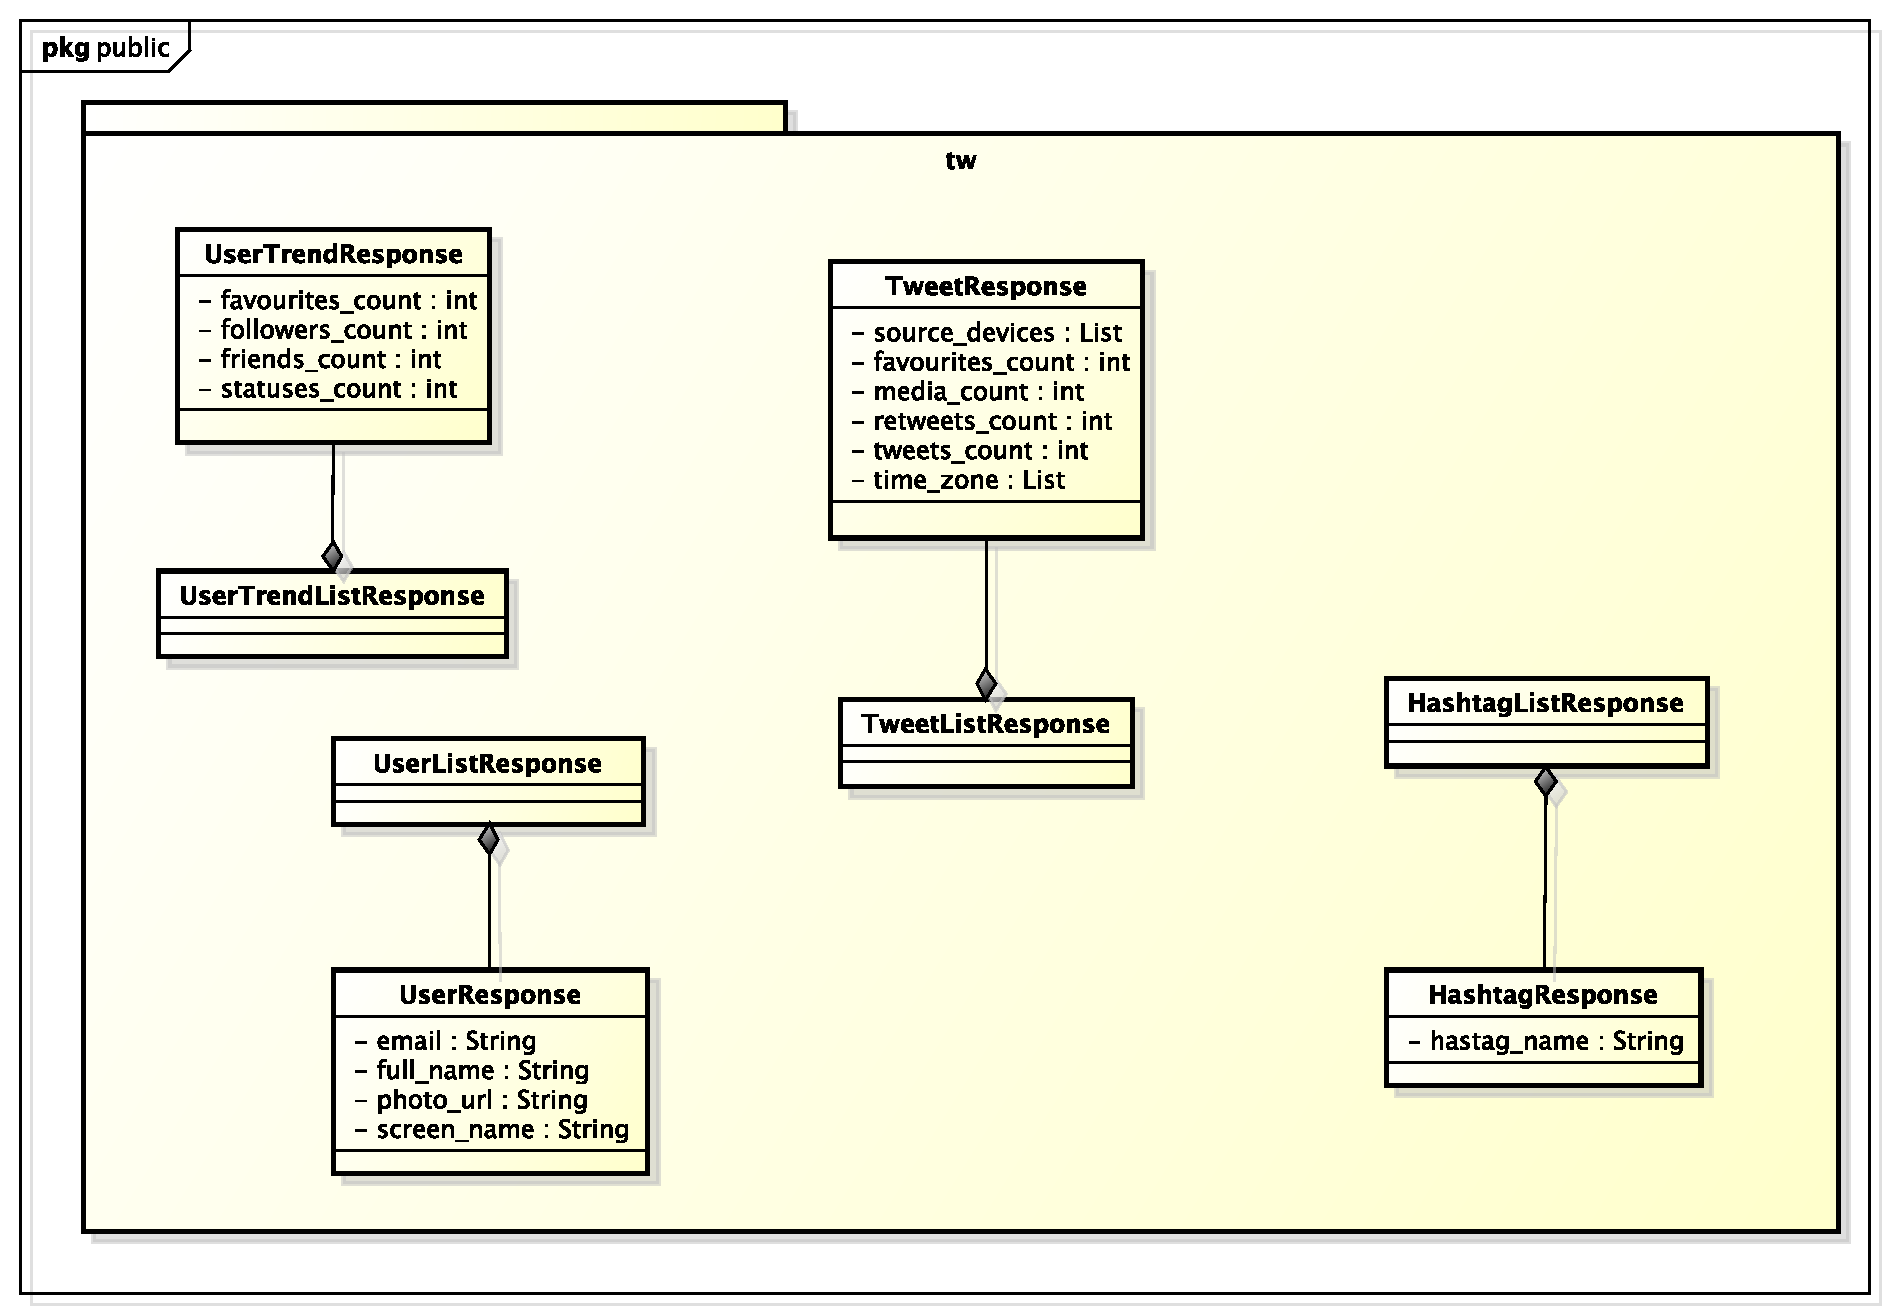
\includegraphics[scale=0.5]{./images/server/resp_tw.pdf}}
	\caption{Package - server::endpoints::resp::public::tw}
\end{figure}

\begin{itemize}
  \item \textbf{Descrizione}: è il package contenente le classi che rappresentano il modello dei dati delle componenti di Twitter da restituire al client;
  \item \textbf{Padre}: server::endpoints::resp::public
  %\item \textbf{Interazione con altri componenti}:
\end{itemize}
% subsubsection

	\paragraph{Classi} % (fold)

    \subparagraph{server::endpoints::resp::public::tw::UserResponse} % (fold)
    \label{subp:bdsm_app_server_endpoints_resp_public_tw_userresponse}
    \begin{itemize}
      \item \textbf{Descrizione}: rappresenta il modello dei dati di un profilo Twitter da ritornare al client;
      \item \textbf{Utilizzo}: viene utilizzata dalle API per restituire la response dei dati di un profilo Twitter al client;
      %\item \textbf{Relazioni con altre classi}:
      \end{itemize}
    % subparagraph bdsm_app_server_endpoints_resp_public_tw_pageresponse (end)

    \subparagraph{server::endpoints::resp::public::tw::UserListResponse} % (fold)
    \label{subp:bdsm_app_server_endpoints_resp_public_tw_userlistresponse}
    \begin{itemize}
      \item \textbf{Descrizione}: rappresenta il modello dei dati della lista di profili Twitter da ritornare al client;
      \item \textbf{Utilizzo}: viene utilizzata dalle API per restituire la response della lista di profili Twitter al client;
      \item \textbf{Relazioni con altre classi}:
        \begin{itemize}
          \item server::endpoints::resp::public::tw::UserResponse
        \end{itemize}
      \end{itemize}
    % subparagraph bdsm_app_server_endpoints_resp_public_tw_userlistresponse (end)

    \subparagraph{server::endpoints::resp::public::tw::UserTrendResponse} % (fold)
    \label{subp:bdsm_app_server_endpoints_resp_public_tw_usertrendresponse}
    \begin{itemize}
      \item \textbf{Descrizione}: rappresenta il modello dei dati dei trend di un profilo Twitter da ritornare al client;
      \item \textbf{Utilizzo}: viene utilizzata dalle API per restituire la response dei trend di un profilo Twitter al client;
      %\item \textbf{Relazioni con altre classi}:
      \end{itemize}
    % subparagraph bdsm_app_server_endpoints_resp_public_tw_usertrendresponse (end)

    \subparagraph{server::endpoints::resp::public::tw::UserTrendListResponse} % (fold)
    \label{subp:bdsm_app_server_endpoints_resp_public_tw_usertrendlistresponse}
    \begin{itemize}
      \item \textbf{Descrizione}: rappresenta il modello dei dati della lista dei trend di un profilo Twitter da ritornare al client;
      \item \textbf{Utilizzo}: viene utilizzata dalle API per restituire la response della lista dei trend di un profilo Twitter al client;
      \item \textbf{Relazioni con altre classi}:
        \begin{itemize}
          \item server::endpoints::resp::public::tw::UserTrendResponse
        \end{itemize}
      \end{itemize}
    % subparagraph bdsm_app_server_endpoints_resp_public_tw_usertrendlistresponse (end)

    \subparagraph{server::endpoints::resp::public::tw::HashtagResponse} % (fold)
    \label{subp:bdsm_app_server_endpoints_resp_public_tw_hashtagresponse}
    \begin{itemize}
      \item \textbf{Descrizione}: rappresenta il modello dei dati di un hashtag di Twitter da ritornare al client;
      \item \textbf{Utilizzo}: viene utilizzata dalle API per restituire la response dei dati di un hashtag di Twitter al client;
      %\item \textbf{Relazioni con altre classi}:
      \end{itemize}
    % subparagraph bdsm_app_server_endpoints_resp_public_tw_hashtagresponse (end)

    \subparagraph{server::endpoints::resp::public::tw::HashtagListResponse} % (fold)
    \label{subp:bdsm_app_server_endpoints_resp_public_tw_hashtaglistresponse}
    \begin{itemize}
      \item \textbf{Descrizione}: rappresenta il modello dei dati della lista degli hashtag di Twitter da ritornare al client;
      \item \textbf{Utilizzo}: viene utilizzata dalle API per restituire la response della lista degli hashtag di Twitter al client;
      \item \textbf{Relazioni con altre classi}:
        \begin{itemize}
          \item server::endpoints::resp::public::tw::HashtagResponse
        \end{itemize}
      \end{itemize}
    % subparagraph bdsm_app_server_endpoints_resp_public_tw_hashtaglistresponse (end)

    \subparagraph{server::endpoints::resp::public::tw::TweetResponse} % (fold)
    \label{subp:bdsm_app_server_endpoints_resp_public_tw_tweetresponse}
    \begin{itemize}
      \item \textbf{Descrizione}: rappresenta il modello dei dati dei tweet di Twitter da ritornare al client;
      \item \textbf{Utilizzo}: viene utilizzata dalle API per restituire la response dei dati dei tweet di Twitter al client;
      %\item \textbf{Relazioni con altre classi}:
      \end{itemize}
    % subparagraph bdsm_app_server_endpoints_resp_public_tw_tweetresponse (end)

    \subparagraph{server::endpoints::resp::public::tw::TweetListResponse} % (fold)
    \label{subp:bdsm_app_server_endpoints_resp_public_tw_tweetlistresponse}
    \begin{itemize}
      \item \textbf{Descrizione}: rappresenta il modello dei dati della lista dei tweet Twitter da ritornare al client;
      \item \textbf{Utilizzo}: viene utilizzata dalle API per restituire la response della lista dei tweet di Twitter al client;
      \item \textbf{Relazioni con altre classi}:
        \begin{itemize}
          \item server::endpoints::resp::public::tw::TweetResponse
        \end{itemize}
      \end{itemize}
    % subparagraph bdsm_app_server_endpoints_resp_public_tw_tweetlistresponse (end)

\subsubsection{server::endpoints::resp::public::ig} % (fold)
\label{ssub:bdsm_app_server_endpoints_resp_public_ig}
\begin{figure}[!htbp]
	\centering
	\centerline{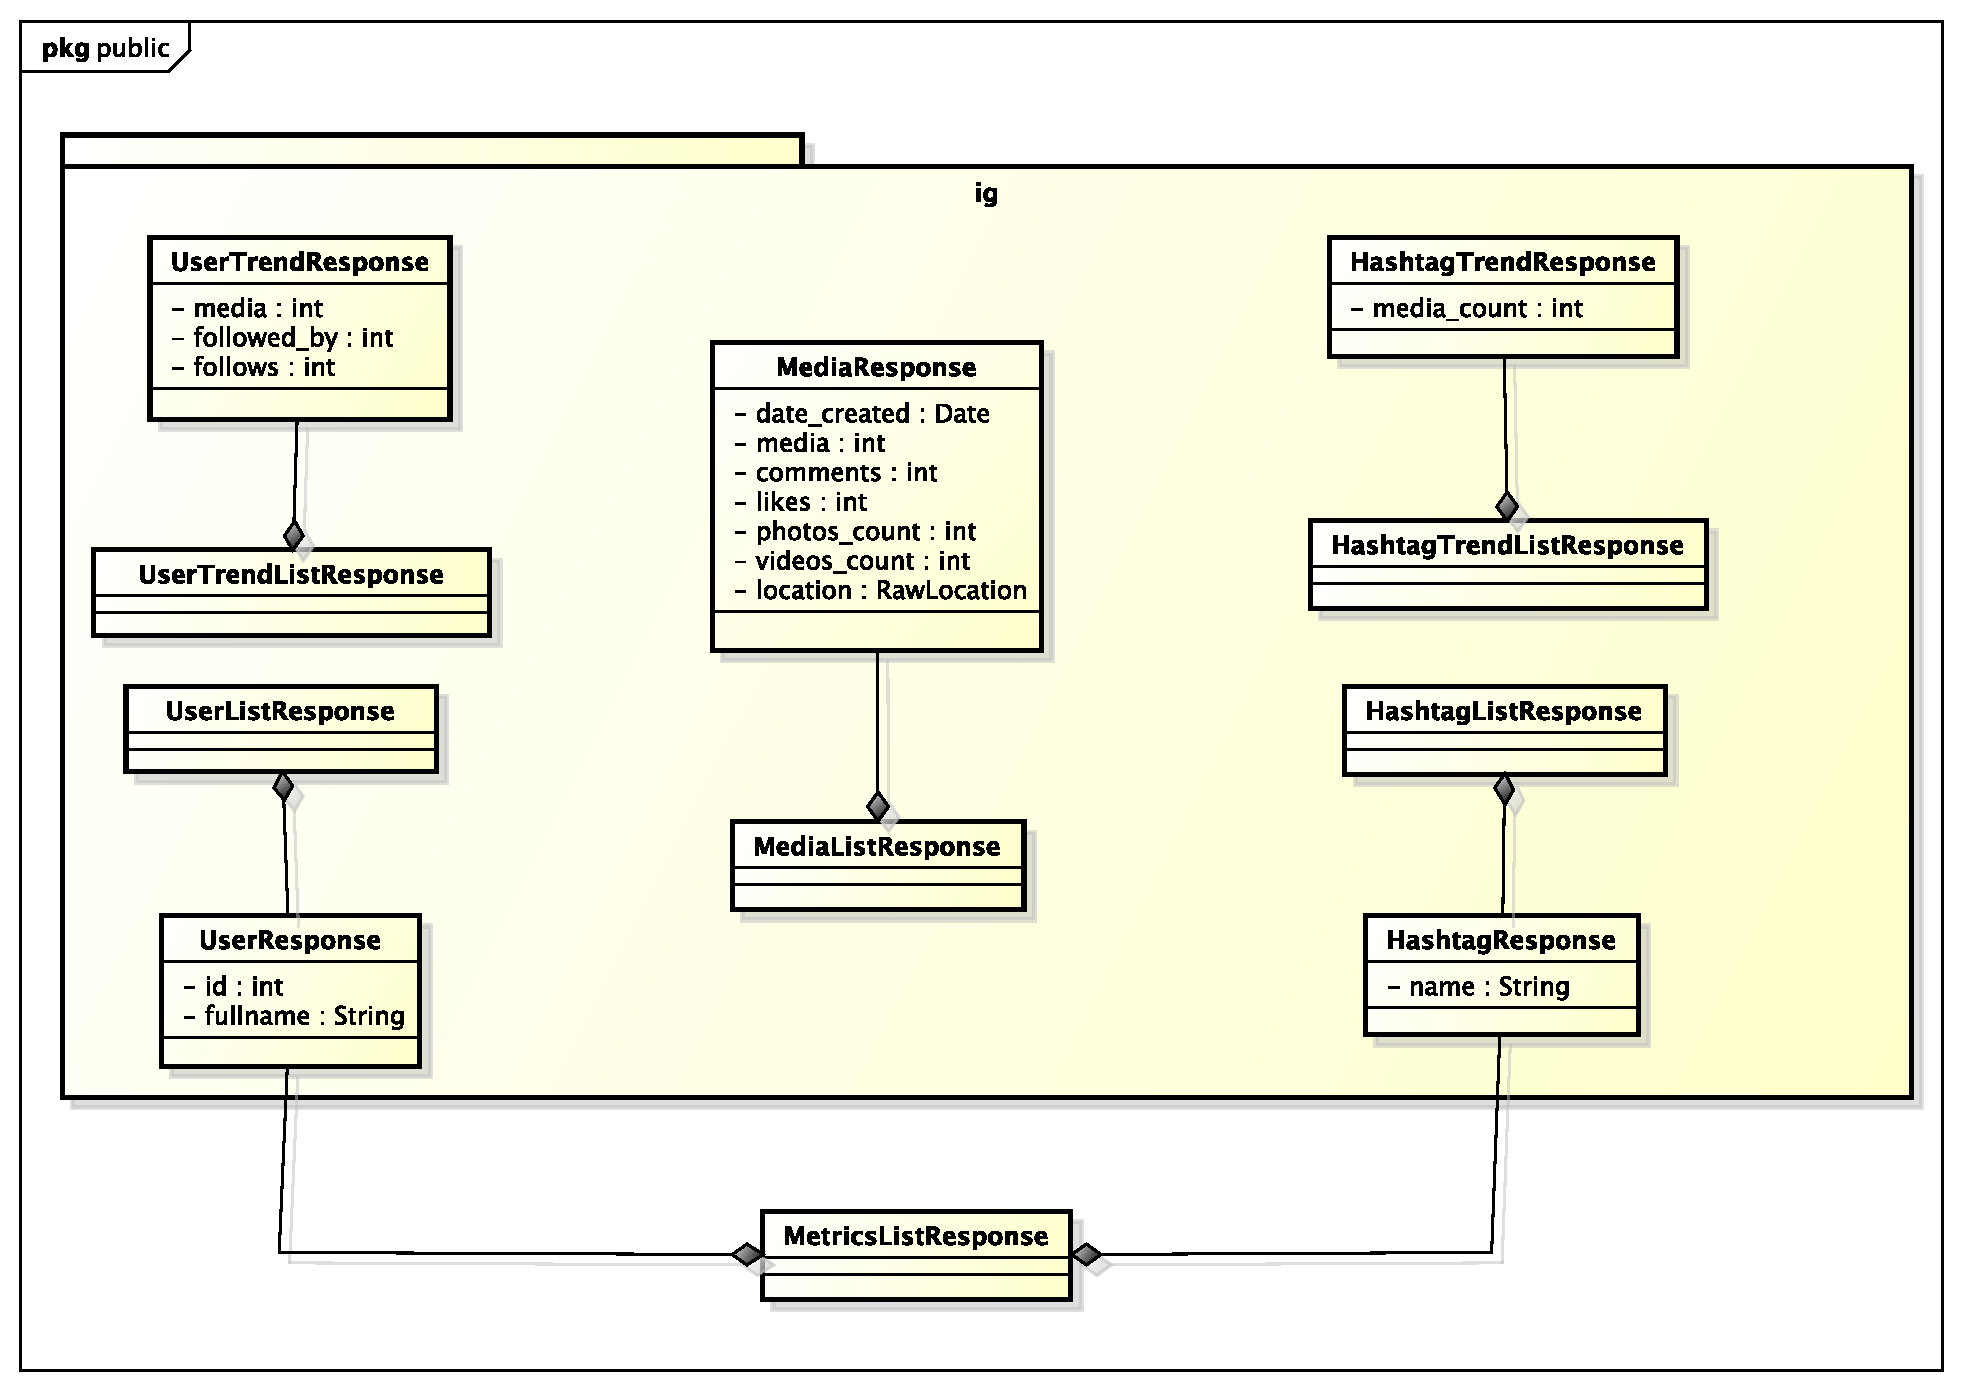
\includegraphics[scale=0.5]{./images/server/resp_ig.pdf}}
	\caption{Package - server::endpoints::resp::public::ig}
\end{figure}

\begin{itemize}
  \item \textbf{Descrizione}: è il package contenente le classi che rappresentano il modello dei dati delle componenti di Instagram da restituire al client;
  \item \textbf{Padre}: server::endpoints::resp::public
  %\item \textbf{Interazione con altri componenti}:
\end{itemize}
% subsubsection

	\paragraph{Classi} % (fold)

    \subparagraph{server::endpoints::resp::public::ig::UserResponse} % (fold)
    \label{subp:bdsm_app_server_endpoints_resp_public_ig_userresponse}
    \begin{itemize}
      \item \textbf{Descrizione}: rappresenta il modello dei dati di un profilo Instagram da ritornare al client;
      \item \textbf{Utilizzo}: viene utilizzata dalle API per restituire la response dei dati di un profilo Instagram al client;
      %\item \textbf{Relazioni con altre classi}:
      \end{itemize}
    % subparagraph bdsm_app_server_endpoints_resp_public_ig_pageresponse (end)

    \subparagraph{server::endpoints::resp::public::ig::UserListResponse} % (fold)
    \label{subp:bdsm_app_server_endpoints_resp_public_ig_userlistresponse}
    \begin{itemize}
      \item \textbf{Descrizione}: rappresenta il modello dei dati della lista dei profili di Instagram da ritornare al client;
      \item \textbf{Utilizzo}: viene utilizzata dalle API per restituire la response della lista dei profili di Instagram al client;
      \item \textbf{Relazioni con altre classi}:
        \begin{itemize}
          \item server::endpoints::resp::public::ig::UserResponse
        \end{itemize}
      \end{itemize}
    % subparagraph bdsm_app_server_endpoints_resp_public_ig_userlistresponse (end)

    \subparagraph{server::endpoints::resp::public::ig::UserTrendResponse} % (fold)
    \label{subp:bdsm_app_server_endpoints_resp_public_ig_usertrendresponse}
    \begin{itemize}
      \item \textbf{Descrizione}: rappresenta il modello dei dati dei trend di un profilo Instagram da ritornare al client;
      \item \textbf{Utilizzo}: viene utilizzata dalle API per restituire la response dei trend di un profilo Instagram al client;
      %\item \textbf{Relazioni con altre classi}:
      \end{itemize}
    % subparagraph bdsm_app_server_endpoints_resp_public_ig_usertrendresponse (end)

    \subparagraph{server::endpoints::resp::public::ig::UserTrendListResponse} % (fold)
    \label{subp:bdsm_app_server_endpoints_resp_public_ig_usertrendlistresponse}
    \begin{itemize}
      \item \textbf{Descrizione}: rappresenta il modello dei dati della lista dei trend di un profilo Instagram da ritornare al client;
      \item \textbf{Utilizzo}: viene utilizzata dalle API per restituire la response della lista dei trend di un profilo Instagram al client;
      \item \textbf{Relazioni con altre classi}:
        \begin{itemize}
          \item server::endpoints::resp::public::ig::UserTrendResponse
        \end{itemize}
      \end{itemize}
    % subparagraph bdsm_app_server_endpoints_resp_public_ig_usertrendlistresponse (end)

    \subparagraph{server::endpoints::resp::public::ig::HashtagResponse} % (fold)
    \label{subp:bdsm_app_server_endpoints_resp_public_ig_hashtagresponse}
    \begin{itemize}
      \item \textbf{Descrizione}: rappresenta il modello dei dati di un hashtag di Instagram da ritornare al client;
      \item \textbf{Utilizzo}: viene utilizzata dalle API per restituire la response dei dati di un hashtag di Instagram al client;
      %\item \textbf{Relazioni con altre classi}:
      \end{itemize}
    % subparagraph bdsm_app_server_endpoints_resp_public_ig_hashtagresponse (end)

    \subparagraph{server::endpoints::resp::public::ig::HashtagListResponse} % (fold)
    \label{subp:bdsm_app_server_endpoints_resp_public_ig_hashtaglistresponse}
    \begin{itemize}
      \item \textbf{Descrizione}: rappresenta il modello dei dati della lista degli hashtag di Instagram da ritornare al client;
      \item \textbf{Utilizzo}: viene utilizzata dalle API per restituire la response della lista degli hashtag di Instagram al client;
      \item \textbf{Relazioni con altre classi}:
        \begin{itemize}
          \item server::endpoints::resp::public::ig::HashtagResponse
        \end{itemize}
      \end{itemize}
    % subparagraph bdsm_app_server_endpoints_resp_public_ig_hashtaglistresponse (end)

    \subparagraph{server::endpoints::resp::public::ig::HashtagTrendResponse} % (fold)
    \label{subp:bdsm_app_server_endpoints_resp_public_ig_hashtagtrendresponse}
    \begin{itemize}
      \item \textbf{Descrizione}: rappresenta il modello dei dati dei trend di un hashtag di Instagram da ritornare al client;
      \item \textbf{Utilizzo}: viene utilizzata dalle API per restituire la response dei trend di un hashtag di Instagram al client;
      %\item \textbf{Relazioni con altre classi}:
      \end{itemize}
    % subparagraph bdsm_app_server_endpoints_resp_public_ig_hashtagtrendresponse (end)

    \subparagraph{server::endpoints::resp::public::ig::HashtagTrendListResponse} % (fold)
    \label{subp:bdsm_app_server_endpoints_resp_public_ig_hashtagtrendlistresponse}
    \begin{itemize}
      \item \textbf{Descrizione}: rappresenta il modello dei dati della lista dei trend di un hashtag di Instagram da ritornare al client;
      \item \textbf{Utilizzo}: viene utilizzata dalle API per restituire la response della lista dei trend di un hashtag di Instagram al client;
      \item \textbf{Relazioni con altre classi}:
        \begin{itemize}
          \item server::endpoints::resp::public::ig::HashtagTrendResponse
        \end{itemize}
      \end{itemize}
    % subparagraph bdsm_app_server_endpoints_resp_public_ig_hashtagtrendlistresponse (end)

    \subparagraph{server::endpoints::resp::public::ig::MediaResponse} % (fold)
    \label{subp:bdsm_app_server_endpoints_resp_public_ig_mediaresponse}
    \begin{itemize}
      \item \textbf{Descrizione}: rappresenta il modello dei dati dei media di Instagram da ritornare al client;
      \item \textbf{Utilizzo}: viene utilizzata dalle API per restituire la response dei dati dei media di Instagram al client;
      %\item \textbf{Relazioni con altre classi}:
      \end{itemize}
    % subparagraph bdsm_app_server_endpoints_resp_public_ig_mediaresponse (end)

    \subparagraph{server::endpoints::resp::public::ig::MediaListResponse} % (fold)
    \label{subp:bdsm_app_server_endpoints_resp_public_ig_medialistresponse}
    \begin{itemize}
      \item \textbf{Descrizione}: rappresenta il modello dei dati della lista dei media di Instagram da ritornare al client;
      \item \textbf{Utilizzo}: viene utilizzata dalle API per restituire la response della lista dei media di Instagram al client;
      \item \textbf{Relazioni con altre classi}:
        \begin{itemize}
          \item server::endpoints::resp::public::ig::MediaResponse
        \end{itemize}
      \end{itemize}
    % subparagraph bdsm_app_server_endpoints_resp_public_ig_medialistresponse (end)

\subsubsection{server::endpoints::resp::private} % (fold)
\label{ssub:bdsm_app_server_endpoints_resp_private}
\begin{figure}[!htbp]
	\centering
	\centerline{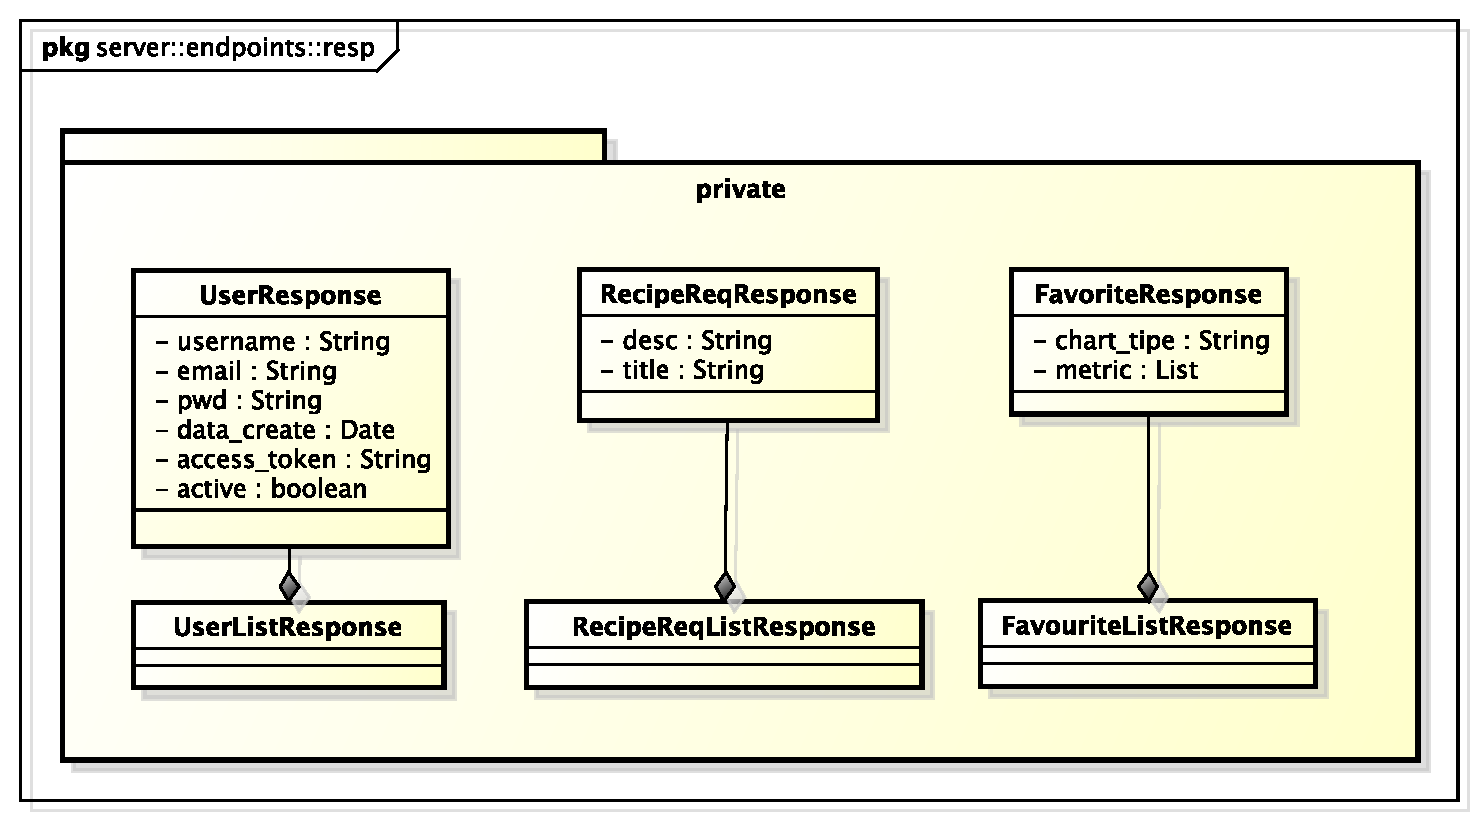
\includegraphics[scale=0.45]{./images/server/resp_private.pdf}}
	\caption{Package - server::endpoints::resp::private}
\end{figure}

\begin{itemize}
  \item \textbf{Descrizione}: è il package che definisce i modelli delle risposte da passare al client in seguito alle chiamate API;
  \item \textbf{Padre}: server::endpoints::resp
  \item \textbf{Interazione con altri componenti}:
  	\begin{itemize}
  		\item server::endpoints::resp::public
	\end{itemize}
\end{itemize}
% subsubsection

	\paragraph{Classi} % (fold)

    \subparagraph{server::endpoints::resp::private::RecipeResponse} % (fold)
    \label{subp:bdsm_app_server_endpoints_resp_private_reciperesponse}
    \begin{itemize}
      \item \textbf{Descrizione}: rappresenta il modello dei dati di una Recipe da ritornare al client;
      \item \textbf{Utilizzo}: viene utilizzata dalle API per restituire la response di una Recipe al client;
      \item \textbf{Relazioni con altre classi}:
        \begin{itemize}
  			\item server::endpoints::resp::public::MetricListResponse
		\end{itemize}
      \end{itemize}
    % subparagraph bdsm_app_server_endpoints_resp_private_reciperesponse (end)

    \subparagraph{server::endpoints::resp::private::RecipeListResponse} % (fold)
    \label{subp:bdsm_app_server_endpoints_resp_private_recipelistresponse}
    \begin{itemize}
      \item \textbf{Descrizione}: rappresenta il modello dei dati di una Recipe da ritornare al client;
      \item \textbf{Utilizzo}: viene utilizzata dalle API per restituire la response di una Recipe al client;
      \item \textbf{Relazioni con altre classi}:
        \begin{itemize}
          \item server::endpoints::resp::private::RecipeResponse
        \end{itemize}
      \end{itemize}
    % subparagraph bdsm_app_server_endpoints_resp_private_recipelistresponse (end)

    \subparagraph{server::endpoints::resp::private::RecipeReqResponse} % (fold)
    \label{subp:bdsm_app_server_endpoints_resp_private_recipereqresponse}
    \begin{itemize}
      \item \textbf{Descrizione}: rappresenta il modello dei dati di una richiesta di Recipe da ritornare al client;
      \item \textbf{Utilizzo}: viene utilizzata dalle API per restituire la response di una richiesta di Recipe al client;
      %\item \textbf{Relazioni con altre classi}:
      \end{itemize}
    % subparagraph bdsm_app_server_endpoints_resp_private_recipereqresponse (end)

    \subparagraph{server::endpoints::resp::private::RecipeReqListResponse} % (fold)
    \label{subp:bdsm_app_server_endpoints_resp_private_recipereqlistresponse}
    \begin{itemize}
      \item \textbf{Descrizione}: rappresenta il modello dei dati di una lista di richieste di Recipe da ritornare al client;
      \item \textbf{Utilizzo}: viene utilizzata dalle API per restituire la response di una lista di richieste di Recipe al client;
      \item \textbf{Relazioni con altre classi}:
        \begin{itemize}
          \item server::endpoints::resp::private::RecipeReqResponse
        \end{itemize}
      \end{itemize}
    % subparagraph bdsm_app_server_endpoints_resp_private_recipereqlistresponse (end)

    \subparagraph{server::endpoints::resp::private::UserResponse} % (fold)
    \label{subp:bdsm_app_server_endpoints_resp_private_userresponse}
    \begin{itemize}
      \item \textbf{Descrizione}: rappresenta il modello dei dati di un utente da ritornare al client;
      \item \textbf{Utilizzo}: viene utilizzata dalle API per restituire la response contenente i dati un un utente al client;
    \end{itemize}
    % subparagraph bdsm_app_server_endpoints_resp_private_userresponse (end)

    \subparagraph{server::endpoints::resp::private::FavoriteResponse} % (fold)
    \label{subp:bdsm_app_server_endpoints_resp_private_favoriteresponse}
    \begin{itemize}
      \item \textbf{Descrizione}: rappresenta il modello dei dati di una View preferita da ritornare al client;
      \item \textbf{Utilizzo}: viene utilizzata dalle API per restituire la response di una View preferita al client;
    \end{itemize}
    % subparagraph bdsm_app_server_endpoints_resp_private_favoriteresponse (end)

    \subparagraph{server::endpoints::resp::private::FavoriteListResponse} % (fold)
    \label{subp:bdsm_app_server_endpoints_resp_private_favoritelistresponse}
    \begin{itemize}
      \item \textbf{Descrizione}: rappresenta il modello dei dati di una lista di View preferite da ritornare al client;
      \item \textbf{Utilizzo}: viene utilizzata dalle API per restituire la response di una lista di View preferite al client;
      \item \textbf{Relazioni con altre classi}:
        \begin{itemize}
          \item server::endpoints::resp::private::FavoriteResponse
        \end{itemize}
      \end{itemize}
    % subparagraph bdsm_app_server_endpoints_resp_private_favoritelistresponse (end)
